\documentclass[../Immersed_Boundary_Method.tex]{subfiles}

\begin{document}

\section{Introduction}

\subsection{The Interpolation Function}

Given the material position $X$ we want to obtian the velocity of fluid at that point. \mn{Note that $X$ usually doesn't lies on the grid point.} This process is directly interpreted by 
\begin{equation}
    \bfu(\mathbf{X}(r, s, t), t)=\int \bfu(\mathbf{x}, t) \delta(\mathbf{x}-\mathbf{X}(r, s, t)) d \mathbf{x}
\end{equation}
\begin{wrapfigure}{l}{0.6\textwidth}
    \centering
    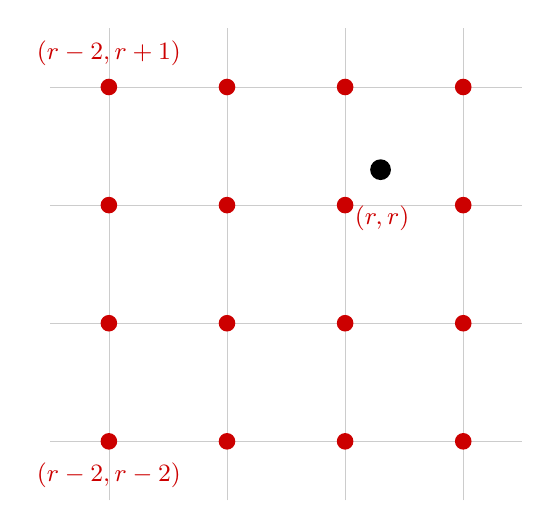
\begin{tikzpicture}[scale=1.5] % Slightly adjusted scale to fit text column better
        % 1. Draw the background grid
        \draw[step=1cm, gray!40, very thin] (-0.5,-0.5) grid (3.5,3.5);

        % 2. Draw the 4x4 grid of red points
        \foreach \x in {0,1,2,3} {
            \foreach \y in {0,1,2,3} {
                \fill[red!80!black] (\x,\y) circle (2pt);
            }
        }

        % 3. Draw the central black dot
        \fill[black] (2.3,2.3) circle (2.5pt);

        % 4. Add the labels
        % Top Left
        \node[red!80!black, above, font=\small] at (0,3.1) {$(r-2, r+1)$};
        % Inner Point
        \node[red!80!black, above right, font=\small] at (2, 1.7) {$(r, r)$};
        % Bottom Left
        \node[red!80!black, below, font=\small] at (0,-0.1) {$(r-2, r-2)$};
    \end{tikzpicture}
\end{wrapfigure}
However in the discrete case we would need the discrete Delta Function. \par

In the figure on the left, black point is the material point and red points are the grid points. The $\delta$ function average all the velocity at the red points. \par

Something to pay attention is that in MATLAB, the convention for a matrix to represent a grid of point is to have lay points with same $x$ coordinat in the \textbf{same row} This may be different from our intuition. However, This is reasonable since we normally define the matrix for storing points to have size 
\[ N_x \times N_y\]
So it has $N_x$ rows. \par

\subsection{Discrete Delta Function}

A commonly used discreted delta function uses a $4 \times 4$ grid. Thus the 1D delta function $\phi(x)$ should support on four points. We have the following postulates:
\begin{enumerate}
    \item $\phi(r)$ is continuous for all real $r$
    \item $\phi(r)=0$ for $|r| \geq 2$
    \item The following gurantee there is no difference between odd index grid point and even index grid point. Since they never exchange information between each others
    \[
    \sum_{j \text { even }} \phi(r-j)=\sum_{j \text { odd }} \phi(r-j)=\frac{1}{2} \text { for all real } r
    \]
    \item The delta function should centered at the origin
    \[
\sum_j(r-j) \phi(r-j)=0 \text { for all real } r
    \]
    \item The $L_2$ norm shoudl be given. 
    \[
    \sum_j(\phi(r-j))^2=C \text { for all real } r
    \]
\end{enumerate}
Here $r \in [0,1)$. This is a standard \textbf{4 point delta function}. We can also have 6 points delta function for higher accuracy. $C$ can be determined by setting $r = 0$. We get 
\[ \phi(r) = \frac{3 - 2r + \sqrt{\Delta}}{8} \qquad \phi(r +1) = \frac{3 - 2r - \sqrt{\Delta}}{8}\]
and 
\[ \phi(r - 1) = \frac{1 + 2r + \sqrt{\Delta}}{8} \qquad \phi(r - 2) = \frac{1 +2r - \sqrt{\Delta}}{8}\]
Here $\Delta = 1 + 4r - 4r^2$. \par
\begin{wrapfigure}{l}{0.6\textwidth}
    \centering
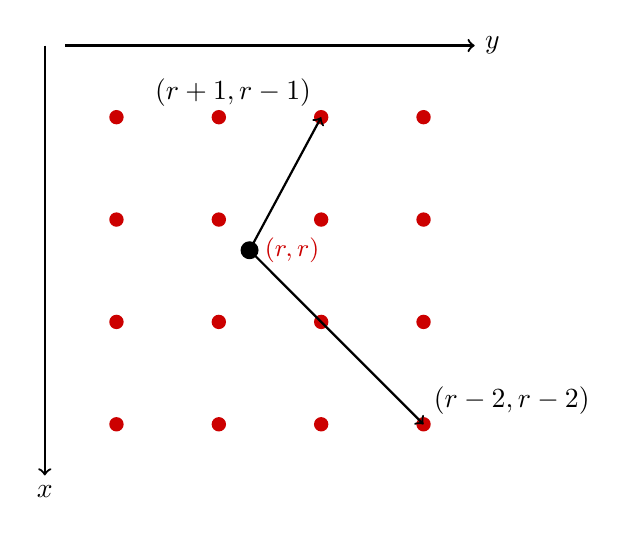
\begin{tikzpicture}[scale=1.3]
    % 2. Draw the grid of red points
    \foreach \x in {0,1,2,3} {
        \foreach \y in {0,1,2,3} {
            \fill[red!80!black] (\x,\y) circle (2pt);
        }
    }
    % 3. Draw the central black dot
    \coordinate (center) at (1.3,1.7);
    \fill[black] (center) circle (2.5pt);

    % 4. Inner Point Label
    \node[red!80!black, right, font=\small, xshift=2pt] at (center) {$(r, r)$};

    % 5. Previous Arrows
    % Arrow to (4,4)
    \draw[->, thick, black] (center) -- (3,0) node[above right] {$(r - 2, r - 2)$};
    % Arrow to (1,3)
    \draw[->, thick, black] (center) -- (2,3) node[above left] {$(r + 1, r - 1)$};

    % 6. NEW: Coordinate Axes (Arrows)
    % Downward arrow on the left (x)
    \draw[->, thick, black] (-0.7, 3.7) -- (-0.7, -0.5) node[below] {$x$};

    % Rightward arrow on the top (y)
    \draw[->, thick, black] (-0.5, 3.7) -- (3.5, 3.7) node[right] {$y$};

\end{tikzpicture}
\end{wrapfigure}
However, in MATLAB, grid points are stored in a particular way. Entries with same $x$ coordinate is in same row and $(0,0)$ is at the upper-right corner. \par

Since the argument for $\phi$ is the position vector of grid point. The value for point $(r-2, r-2)$ is actually at the lower right as shown in the picture on the left. \mn{I made a mistake here when writing the function \texttt{twoD\_delta\_function}. The order is incorrect. Time: 251212}


\end{document}